% multipath execution on a large distributed microarchitecture
%
%\documentclass[10pt,twocolumn,dvips]{article}
\documentclass[10pt,dvips]{article}
\usepackage[english]{babel}
\usepackage{epsfig}
%
%\usepackage{fancyheadings}
%\usepackage[T1]{fontenc}
%\usepackage[latin1]{inputenc}
%
%\usepackage{twocolumn}
%\usepackage{verbatim,moreverb,doublespace}
%\usepackage{rotate,lscape,dcolumn,array,rotating,latexsym}
%
%\input{epsf}
%
\textwidth 6.5in
\textheight 9.0in
\topmargin -0.6in
\oddsidemargin 0mm
\evensidemargin 0mm
%
%\pagestyle{empty}
%
\begin{document}
\parskip 2mm
%
%
\title{Multipath Execution on a Large-Scale Distributed 
Microarchitecture}
%
\author{
A. Khalafi, D. Morano, D.R. Kaeli\\
Northeastern University\\
{akhalafi, dmorano, kaeli}@ece.neu.edu\\
\and
A.K. Uht \\
University of Rhode Island\\ uht@ele.uri.edu
}
%
\maketitle
%\thispagestyle{empty}
%
\begin{abstract}
This paper explores the implementation of multipath execution on a
large distributed microarchitecture.  Larger microarchitectures can
speculatively execute possibly several hundreds of instructions
simultaneously.  This provides a means to extract larger amounts of
instruction level parallelism even from programs that are very
sequential in nature.  However, conditional branches present a
difficult challenge when a very large number of speculative
instructions have to be squashed as a result of a mispredition.
Multipath execution is a means to address this problem
by avoiding or reducing the penalties of some branch mispredictions when
instrcutions from both outcomes of the branch were
already executed within the core of the processor.

We briefly present the outline of a large-scale distributed
microarchitecture and discuss how we overlay multipath execution on
it.  We provide simulation results for several microarchitectural
configurations that demonstrate the positive effects of multipath
execution in reducing the penalties associated with branch
mispredictions.
\end{abstract}
%
\section{Introduction}
%
Performance penalties due to mispredicted branches continue to
present a challenge for achieving higher performance execution
of single threaded programs.
These penalties restrict the instruction level parallelism (ILP)
that might be achieved unless they can be reduced.
One approach towards reducing the negative effects of mispredicted
branches, and a moderately successful one, has been the pursuit
of better branch predictors.  However, many branches in typical
programs remain difficult to predict accurately and these continue
to limit performance in many codes.

Another approach towards mitigating the effects of mispredicted branches
has been that of attempting to address the problem of executing
down both paths of a branch in some measure or another before the
branch is able to resolve.  This approach is not new but presents
complexity problems that have made it less than attractive for
many practical processor designs.  However, with the advent of ever
increasing amounts of speculative execution, the need to address
the problems associated with mispredicted branches has only grown worse.

Current commercial machines only allow for modest
amounts of speculative execution (usually several instructions to 
less than about 40 instructions per thread).
However, for those computer applications that demand it,
future machines may need to execute upwards of one hundred to
several hundreds of instructions speculatively in order to maximize
execution performance.  This trend will only increase the pressure to try
and reduce the effects of branch mispredictions.

Our work presented in this paper is oriented towards reducing the
negative effects of mispredicted branches through multipath execution
while doing so on an aggressive large-scale (able to speculatively execute
possibly hundreds of instructions simultaneously)
distributed
microarchitecture.  
A large microarchitecture offers the
possibility to significantly step up program speedups through 
the exploitation of ILP.
However, many problems common to more conventional processor designs
are either at least as difficult to deal with on a large-scale
microarchitecture or indeed become more difficult to deal with.
The problem of mispredicted branches is one of these latter problems.
The penalty associated with a mispredicted branch can now mean
the possible squashing and associated opportunity lost of possibly
hundreds of instructions that were in flight.  

Another issue that arises in large-scale microarchitectures is the
problem of efficient execution resource usage.
As we may speculatively execute many branch paths ahead of execution
commitment, the likelihood
of the most recent (latest) speculatively executed instruction to
be committed (part of the program's committed execution trace) tends
towards zero.  This occurs because as each new speculative branch is
encountered, speculative execution continues down one of its
outgoing paths.  The probability of commitment for instructions on 
that outgoing
path is the product of the probability that
the branch will be committed, times the probability of that branch's outcome.
The product of the probabilities of all speculative branch outcomes
eventually approaches zero after a certain
number of speculative branches are visited. 
At a certain point, the likelihood of the committed (correct)
program execution to proceed down an alternative program path,
besides the one defined by each sequential predicted branch outcome,
becomes greater.  This would indicate that for very large speculative
machines, multi-path execution is all but a necessity to most
efficiently allocate and use the available execution resources.

Our present work on multipath execution is part of a larger
desire to explore large-scale ILP speedups in sequential programs.
This goal has been motivated through the work of researchers like
Lam and Wilson ~\cite{Lam92},
Uht and Sindagi ~\cite{Uht95},
Gonzalez and Gonzalez ~\cite{Gon97}.
In this paper, we briefly present an overview of our large-scale distributed
microarchitecture suited for achieving large ILP speedups.  
We then propose a strategy for handling
multipath execution on this microarchitecture.

The rest of this paper is organized as follows.
Section 2 provides some background on multipath execution.
In section 3, we provide some analysis of the conditional
branches in some benchmark programs.  
Section 4 presents an overview of our large-scale distributed
microarchitecture.
We will also discuss how we
would like to 
spawn speculative execution paths
in response to certain conditional branches that 
are encountered.
Section 5 presents some simulation results for various
configurations of our machine and how multipath execution
changes the results when applied.  Shown first are simulation
results for various machine configurations when execution is in
single path mode only.  We then show results for
the same benchmark suite with varying numbers of additional
speculative execution paths.
We summarize and conclude in section 6.
%
\section{Background on Multipath Execution}
%
Early work on multipath execution was
dominated by IBM in the
late 1970s and 1980s \cite{Conners79}.
The earliest attempts at multipath
execution started with the ability to prefetch down both
outcomes of a conditional branch.  This became more aggressive
to the point of actually executing down both outcomes of
a conditional branch.  Aggressively executing down both outcomes
of conditional branches has been explored in work such as that by
Wang \cite{Wang90}.  
More aggressive research by Uht and
Sindagi \cite{Uht95} explored the intersection of both
multipath execution and future large-scale microarchitectures
capable of possibly hundreds of instructions being executed simultaneously.
They also addressed the general question of speculatively executing
more than two paths simultaneously.
Work on dual path execution (only two speculative paths) has
been done by Heil and Smith~\cite{Heil96}.
Examining multipath execution on the PolyPath microarchitecture,
Klauser et al explored several implementation details
as well as demonstrating an improvement of three speculative paths
over just having two.

An increasingly attractive approach to multipath execution is that
of using a basic simultaneous multi-threaded (SMT) processor
to provide the resources for essentially executing multiple paths
of a single architected program thread.  This work follows from
the original SMT idea and followed from the work by
Tullsen et al~\cite{Tullsen96}.  
The work by Tullsen et al focused
on making better use of the processor when
branch mispredictions are encountered by filling processor resources with
work from other architected threads following a misprediction.
An extension of this idea is to use resources for executing
the alternative path (not predicted path) of a mispredicted branch.
An example of this approach has been discussed by 
Wallace et al \cite{Wallace98}.  This general approach of combining
both simultaneous multithreading with multipath execution appears
to be a good compromise to the problem of most efficiently using
processor resources.  This approach also lends itself towards
hardware that possibly can be programmed at run-time for providing either
maximum single threaded execution speed or maximum multithreaded throughput.

Ahuja et al \cite{Ahuja98} explore some limits for speedups from
multipath execution but their work is still largely restricted to more
conventional (modest sized) microarchitectures with less than approximately
128
speculative instructions in flight.  Our present work explores the use
of multipath execution on a significantly larger microarchitecture than
that of Ahuja or the other past work with the exception of that by
Uht and 
Sindagi \cite{Uht95}.
Our present work is capable of having several hundred or more
speculative instructions in flight and is most patterned after the
work by Uht.
%
\section{Conditional Branch Characterization}
%
Since the proper handling of conditional branches is important
in any microarchitecture that spawns additional speculative
paths for unresolved branches, some attention is given
towards characterizing their behavior.  
We focused
on five benchmark programs for characterizing branch behavior.
The benchmark programs explored along with some statistics 
are given in Table \ref{tab:benches}.

\begin{table}
\begin{center}
\caption{Benchmarks Analyzed and Some Statistics.}\label{tab:benches}
\begin{tabular}{|c|c|c|c|c|}
\hline 
benchmark&
prediction accuracy&
avg. L1 miss rate&
dynamic cond. brach-es & forward branches\\
\hline
\hline 
go&
72.1\%&
96.6\%&
9.0\% & 89\%\\
\hline 
gap&
94.5\%&
98.9\%&
6.2\% & 91\%\\
\hline 
bzip&
90.5\%&
98.5\%&
7.0\%&81\%\\
\hline 
gzip&
85.4\%&
97.0\%&
8.8\%&85\%\\
\hline 
parser&
92.6\%&
98.3\%&
13.0\%&85\%\\
\hline
\end{tabular}
\end{center}
\end{table}

The {\tt go} benchmark is from the SpecInt-95 suite while the rest
are from the SpecInt-2000 suite.
All benchmark programs were executed for 100 million instructions
as a warm up for the simulator.  After this they were simulated
for 500 million instructions for which all data was collected.
The predictor used was a PAg with
a PBHT of 1024 entries and a GPHT size of 4096 entries.
The L1 cache was a 32kB, 2-way set associative, with 1 cycle hit
penalty and a 20 cycle miss penalty.

We were interested
in the size of the branch domains for both all branches
dynamically executed in the programs as well as for those branches 
that contribute most to mispredictions.  The branch domain size
is the number of instructions on the not-taken output path
before a join with the target instruction of the branch.
Figure \ref{fig:numbranches} shows a probability distribution of
the percentage of the number of dynamic branches that occur at
or below a branch domain size.  
Figure \ref{fig:mispredictions} shows a probability distribution of
the number of branch mispredictions versus
branch domain size.
From these two figures it can be seen 
that a large fraction of total mispredictions 
is due to branches with small domain
sizes. 
This is likely a valuable characteristic to exploit for
possible alternative speculative paths in our proposed
microarchitecture.  This is so since all of the branch domain
instructions for most
branches will be issued into the execution window allowing
for both branch outcomes to be executed simultaneously
in our microarchitecture.
To get a better understanding of how to handle different branches,
we proceeded to define four orthogonal characteristics
for conditional branches that might give us insight into
how they might be handled in the microarchitecture.
The four characteristics used to classify each conditional branch are :

\begin{figure}
\vspace{0.2 in}
\setlength{\epsfxsize}{10cm}%7
\centerline{\epsfbox{numbranches.eps}}
%\centering
%\epsfig{file=numbranches.eps,width=5.8in}
\caption{{\em Probability Distribution For Dynamic Branches versus
Branch Domain Size.} 
Shown are the number of dynamic branches versus branch domain size
in instructions.}
\label{fig:numbranches}
\end{figure}

\begin{figure}
\vspace{0.2 in}
\setlength{\epsfxsize}{10cm}%7
\centerline{\epsfbox{mispredictions.eps}}
%\centering
%\epsfig{file=mispredictions.eps,width=5.8in}
\caption{{\em Probability Distribution For Branch Mispredictions
versus Branch Domain Size.} 
Shown are the dynamic branch mispredictions versus 
branch domain size
in instructions.}
\label{fig:mispredictions}
\end{figure}

\begin{itemize}
\item{execution frequency}
\item{branch predictability}
\item{direction of the branch target -- forward or backward}
\item{distance to the target of the branch}
\end{itemize}   

We classify each conditional branch as 
being either a high dynamic frequency branch
or a low dynamic frequency branch.  
If the conditional branch
is within the top 90\% of all dynamically executed conditional branches,
it is classified as a \textit{high} frequency branch, else it 
is \textit{low} frequency.
For each conditional branch, we also accumulate statistics on
its predictability.  Figure \ref{fig:bpdist} shows 
the distribution of branches versus prediction accuracy.
As can be seen, for most benchmarks
the branche predictability is distributed over a large range of values.
One implication of this is that we need to target most of branches 
regardless of their predictability.

The other parameter that is also recodrded is the direction of the branch 
whihc can simply
be either a 
\textit{forward} branch or a 
\textit{backward} branch.
Finally, the distance of the branch to 
the instruction at the
branch targer is computed and recorded.  The distance is measured
in instructions.  If the target of the branch is less than 170 instructions
from the branch itself, the branch is considered to have a 
\textit{near} target, else it is considered to have a
\textit{far} target.  The value of 170 instructions was chosen
because for many of the machine configurations that we will be
investigating, this number is approximately between one half of
the possible number of speculatively executed instructions
that can be in-flight and two thirds of the total possible number.
This will be clarified later.

\begin{figure}
\vspace{0.2 in}
\setlength{\epsfxsize}{10cm}%7
\centerline{\epsfbox{bpdist.eps}}
%\centering
%\epsfig{file=bpdist.eps,width=5.8in}
\caption{{\em Probability Distribution of Branches versus Prediction Rate.} 
Shown are the percentage of dynamic
branches with a predictability at or less than ia given prediction
accuracy.}
\label{fig:bpdist}
\end{figure}
%
\section{A Large-scale Distributed Microarchitecture}
%
Our primary goal is to converge on a microarchitecture suitable
for extracting large ILP speedups from sequential programs.
This has resulted so far in a very aggressive large (and scalable)
microarchitecture capable of having many hundreds or perhaps thousands
of speculatively executed instructions in flight.  Scalability
of the microarchitecture is achieved through its distributed nature.
In general, scalability requires little to no dependence on major
central microarchitectural hardware structures in the machine.
This goal presents many challenges (not further enumerated here)
to say the least but the efficient handling of multipath execution
is one of those challenges.  

Future microarchitectures also need to 
address many associated issues surrounding conditional branches.
Spawning alternative speculative paths when encountering conditional
branches is just one aspect of handling the consequences of
unresolved control flow.
In addition, exploitation
of control
and data independent instructions beyond the join of a branch should
also be capitalized upon where possible.
Further, choosing which paths in multipath execution should
be given priority for machine resources is also a necessary concern.
As shown by Uht and Sindagi ~\cite{Uht95},
equal priority to all simultaneous paths
of a program is not the most efficient use of hardware resources.
In our microarchicture we will refer to the most predicted path
in a program as the 
\textit{mainline} path.  
This path corresponds to the single speculatively
executed path in most conventional superscalar processors.
In our microarchitecture,
we give execution resource priority to this mainline path with respect
to any possible alternative speculative paths.  
Since additional speculative paths have lower priority with
respect to the mainline (most predicted) path, they are often referred
to as being
\textit{disjoint} paths.  
The term \textit{disjoint} refers to that fact that the assignment
of execution resources for that path is likely (and should likely) be
deferred in time
as compared with when execution resources are assigned to the mainline
path.
This term is taken from Uht's 
1995 work ~\cite{Uht95}.

Figure \ref{fig:disjoint} shows a typical program fragment that
highlights some aspects of what we would like our microarchitecture
to address.
Mainline path execution (the most predicted path) is shown with the
solid bold control flow edges.  Opportunities for the spawning of alternative
speculative paths (disjoint paths) are shown with the lighter dashed
control flow edges.  In this example, two simple, single-sided hammock 
branches are shown in the body of the loop.  One is predicted as
being taken.  The other is predicted to fall through.  Our microarchitecture
will try and exploit both types of conditional branches by capturing
and speculatively executing
all of the instructions in the body of this loop (given this particular
case).  This is possible due to the ability of the microarchitecture to
both execute large numbers of instructions speculatively but also
because our microarchitecture is specially suited towards handling
issues related to multipath execution.

\begin{figure}
\centering
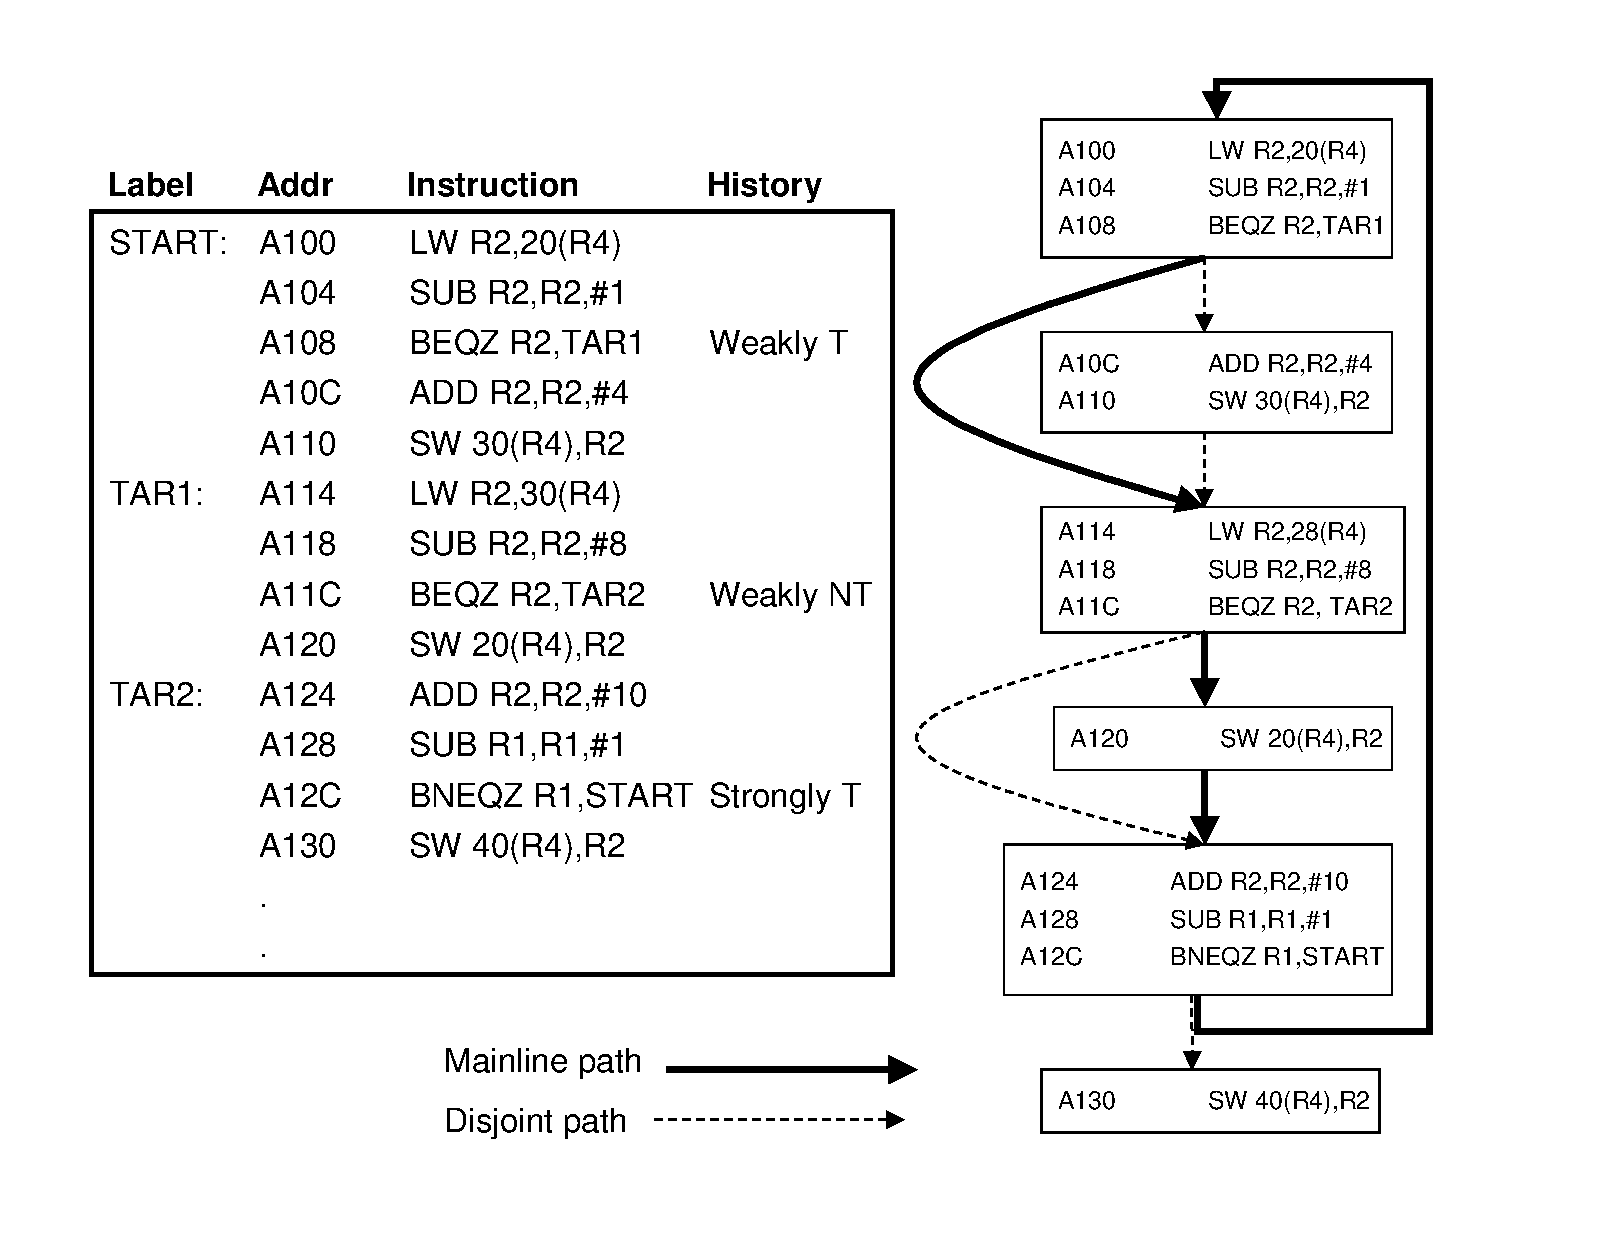
\epsfig{file=disjoint.eps,width=4.5in}
\caption{{\em Example Program Showing Predicted and Disjoint
Paths.} 
This example shows both the predicted path through the program 
(in bold) as
well as where alternative speculative disjoint paths may be
spawned (dashed).}
\label{fig:disjoint}
\end{figure}

A brief overview of our general
large-scale distributed microarchitecture is presented in the next
subsection.  A brief general discussion of the basic operation
of the machine follows and a discussion of the specific handling
of conditional branches is addressed after that.
%
\subsection{Basic Microarchitecture Components and Layout}
%
In this section we present the basic components of our proposed
microarchitecture along with some of their interconnections.
An overall high-level view of the core of our microarchitecture is shown in 
Figure \ref{fig:window}.

\begin{figure}
\vspace{0.2 in}
\setlength{\epsfxsize}{10cm}%7
\centerline{\epsfbox{window.eps}}
%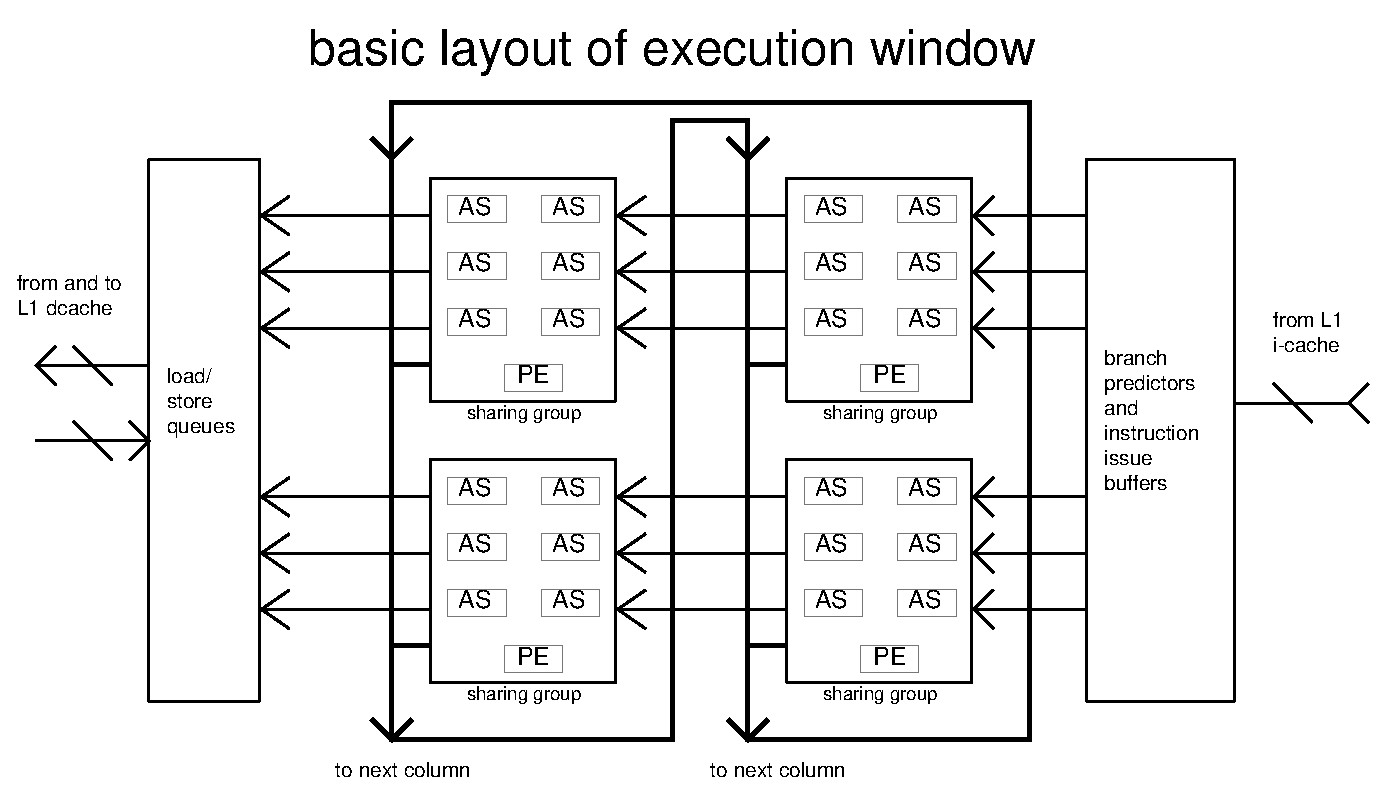
\epsfig{file=window.eps,width=5.8in}
\caption{{\em High-level View of the Distributed Microarchitecture.} 
Shown is a layout of the Active Stations and Processing Elements
along with some bus interconnections to implement a large,
distributed microarchitecture.}
\label{fig:window}
\end{figure}

We have extended the idea of Tomasulo's reservation
station \cite{Tom67} to provide the basic building block for a distributed
microarchitecture.  Tomasulo's reservation station provided for the
simultaneous execution of different instructions over several
functional units.  
Register results from the functional units were placed on
a common data bus and looped back to provide source register operands 
for instructions waiting in the reservations stations as well as
for updating of the register file.  In our microarchitecture,
output results are not looped back to the inputs of the reservations
that provided the results but are rather forwarded to a new set of
stations that form a new spatially separate group from the first.  
We
also extend the idea of the reservation station to allow for multiple
executions (re-executions) of the same instruction in the station.  We
keep instructions in their associated stations station until they are
retired (either committed or squashed).  We call our adaptation of the
reservation station the \textit{active station} (\textit{AS}).

Rather than lay the active stations out in silicon simply next to
function units that will execute the instructions issued to them
(like with the original reservation station idea),
we lay them out in a two dimensional grid whereby sequentially
issued instructions will go to sequential ASes down a column of
the two dimensional grid of ASes. 

Dispersed among the active stations are associated execution
units.  These executions units are represented in the figure as
a \textit{processing element} (\textit{PE}).  
Although an AS always only holds at most a single instruction,
PEs may consist of a unified all-purpose execution unit capable of
executing any of the possible machine instructions or
several functionally partitioned units individually tailored
for specific classes of instructions (integer ALU, FP, or other).

Groups of active stations along with their associated processing
element
are termed \textit{sharing groups}.  Sharing groups somewhat resemble
the relationship between the register file, reorder buffer,
reservation stations, and function units of most conventional
microarchitectures.  They have a relatively high degree of bus
interconnectivity between them as conventional microarchitectures do.
In our case, the active stations serve the role of both the
reservation station and the reorder buffer of more conventional
machines.

A scalable interconnect fabric 
is provided to forward result
operands from earlier active stations to latter active stations in
program order.  Result operands consist of register, memory, and
instruction predicates.  We also employ a strategy of predicating all
issued instructions within the microarchitecture itself.  This is also 
invisible from the instruction set architecture of the machine.
The interconnect fabric is simply shown by
the bold vertical buses in the figure.  These result-forwarding buses
loop around from the bottom of left adjoining columns to the tops of
the right adjoining columns.  The forwarding from the far lower right
also loops around to the far upper left.  In all, the forwarding
buses (interconnection fabric) form the characteristic ring pattern
passing by each sharing group in the execution window.
It should be noted that the interconnection fabric is not
entirely passive (or else the microarchitecture would not
scale to large sized) but rather is an active network.
Several active networks are possible.  We used a simple one
in the present work where a group of four parallel buses transport
result operands to subsequent sharing groups.  The buses are repeated
at a fixed interval of every four sharing groups.

The less bold horizontal buses
form the paths by which instructions are issued to active stations
from the decoded instructions buffers, shown on the far right.
Variations in instruction buffers are possible and may be thought
to resemble trace caches or a sort.
Finally, on the far left, horizontal buses take committed program
stores from retired store instructions residing in the active stations
to the load/store queues (one per row).
The two dimensional
grid of active stations along with their interspersed processing elements
is termed the \textit{execution window}.

The example 
machine configuration
of Figure \ref{fig:window}, 
consists of 
two columns of sharing groups.  Each sharing group contains two columns of
active stations (the specific use of which is explained later).
Each sharing group also contains three rows of active stations
and a single processing element in the shown case.  
We generally characterize
a basic machine configuration according to the triple: sharing group
rows, active station
rows per sharing group, and sharing group columns.  We normally
show these numbers concatenated with a hyphen so that the machine shown
in the figure, as an example, would be abbreviated {\tt 2-3-2}.

The instruction fetch unit (not shown) is responsible for
fetching instructions from the memory hierarchy, these are then decoded
and placed into the issue buffers.   
Currently, branch predictors are provided one per AS row of the execution
window.  
They are located between the issue buffers and the buses that feed
decoded instruction information into the execution window and the
active stations.  
The branch predictions flow along with
the decoded instruction itself into the
execution window when instructions are issued to the active stations.
Updates of the branch predictors come from resolved branches
of the same row that they each serve.

Not shown in the Figure, and outside of the execution window,
lies address-interleaved L1 instruction and data caches, along with
interleaved L2 I/D caches and finally, interleaved main memory.
Interleaving of the entire memory subsystem is generally necessary
to provide sufficient bandwidth for instruction fetching and the
enhanced load bandwidth needed for large sized machines.
%
\subsection{Basic Machine Operation}
%
Instructions are fetched from memory, decoded, and staged in buffers
(not too dissimilar from trace caches).  Variation in fetch buffer
design has been considered but it is not discussed in more detail here.
When an entire column
of active stations is free to accept new instructions, generally
an entire column of instructions are issued to the free active station
column from a fetch buffer.
Conditional branches are
predicted at or just before instructions issue to the ASes.
The prediction of the branch outcome 
prediction is sent along with the
decoded instruction information when instructions are issued to
ASes.

All of the active stations in a given column are issued instructions
in a single clock.  
In our present implementation, newly issued instructions
are only issued to a single column of active stations within
a column of sharing groups.  The other column of active stations
in our current sharing groups (which currently have a total
of two columns of ASes) is reserved for the spawning of additional
execution paths as a result of a condition branch instruction.
When and how additional paths are spawned is discussed later.

It should be noted that there are several strategies for
issuing instructions to available active station columns.
Since all issued instructions are speculative, instructions
from either outgoing path of a conditional branch can be issued
to sequential active stations.
The fetch unit is responsible for preparing for such decisions.
Even when a conditional branch is predicted as being taken,
instructions may still be issued sequentially down the not-taken
path under most circumstances.  If the distance to the target 
of a branch
that is predicted to be taken is not too large,
instructions may be issued along the program static order (or not-taken
path) of the branch in the hopes of capturing hammock styled branch
constructs.  A more detailed discussion on these alternatives is
presented later in the paper.

Program dependencies (control, register, and memory) are 
maintained through the use of tags that
are associated with all forwarded operands.
This has some resemblance to register tags used in more conventional 
microarchitectures but has been more generalized for use in this
distributed microarchitecture.  Instructions remain in their
associated active stations until they are retired by either being
committed or abandoned (squashed).  In this way, the active stations
(or rather the whole set of them)
fulfill the role of the reorder buffer or register update unit of more
conventional microarchitectures.
The exact details of the enforcement of program dependencies
is not covered further in this paper.

Much more detailed information about this microarchitecture
can be found in a technical report by Uht et al~\cite{Uht01}.
Additionally, a more detailed discussion of the mechanism used for
enforcing program dependencies in this microarchitecture
can be found in a report by Kaeli et al~\cite{Kaeli01}.
A more detailed discussion about multipath spawning is given
in the following section.
%
\subsection{Machine Handling of Conditional Branches}
%
The run-time machine microarchitecture only has limited information
available to it for making certain optional decisions.
There are two major alternatives that the machine needs to constantly
consider.  The first is whether to issue instructions to sequential
ASes following
the not-taken path of the condition branch or to issue instructions
along the 
taken path.  
The second major decision to make is
whether to spawn an alternative speculative path
on any given conditional branch.
The machine only has the following information
available at run-time for making microarchitectural decisions :

\begin{itemize}
\item{distance to the target of the branch -- near/far}
\item{branch target direction -- forward/backward}
\item{the branch outcome prediction}
\end{itemize}   

Branches with \textit{near} targets are those where
the distance from the branch to the target is smaller than
the total number of instructions that the machine can have
in-flight simultaneously.  All other branch targets are considered
\textit{far} targets.

First, if a backward branch is predicted taken,
we will speculatively follow it and continue issuing instructions
into the execution window for the mainline path from the target
of the branch.  
For a backward branch that
is predicted not-taken, we continue issuing following the
not-taken output path.

If a forward branch has a near target (small domain size), then we
issue instructions from the domain of the branch (following the
not-taken output path) whether or not it is the most predicted path.
Our mainline path continues along the predicted branch output path
regardless of whether it was the taken or not-taken one.  
We spawn a disjoint
alternative path for the opposite output of the branch from
the mainline path case, whatever it is.
This action
provides the benefit of having both the domain and target of the branch
in the execution instruction window of the machine.  

For forward branches with a far target,
if the branch is predicted taken, we issue following the target
of the branch.  If the branch is predicted not-taken, we continue
issuing instructions for the mainline path following the not-taken
outcome of the branch.  In both of these cases, we do not
spawn an alternative path for this branch.
%
\section{Simulation Results}
%
We present results from simulations of a set of machine configurations
using the general microarchitecture described previously.
We first describe something about our simulation process.
We then present simulations for five benchmark programs
on six different machine configurations.
%
\subsection{Methodology}
%
The simulator is a recently built tool that shares some similarity
to SimpleScalar \cite{Austin97} but which was not based on it.
We execute
SpecInt-2000 and SpecInt-95 programs on simulated machines
that feature a MIPS-1 ISA along with the addition of some MIPS-2 and
MIPS-3 ISA instructions.  We are using the standard SGI Irix system
libraries so we needed some MIPS-2 and MIPS-3 instructions to accommodate
that.  All programs were compiled on an SGI machine under Irix 6.4 and
using the standard SGI compiler and linker.  The code was compiled with
standard optimization ({\tt -O}) for primarily the MIPS-1 ISA ({\tt -o32}).
%
\subsection{IPC Results and Discussion}
%
The data below are IPC results for various sized configurations of
the machine.  Six machine configurations were simulated.
The numbers of each of the major machine components, for each of the six
simulated configurations, are given in Table \ref{tab:configs}.

\begin{table}
\begin{center}
\caption{Machine configurations simulated for each of the benchmark
programs.}
\label{tab:configs}
\begin{tabular}{|c|c|c|c|}
\hline 
config&
SG rows&
ASes per SG&
SG columns\\
\hline
\hline 
1&
8&
4&
16\\
\hline 
2&
8&
4&
8\\
\hline 
3&
8&
8&
8\\
\hline 
4&
8&
8&
16\\
\hline 
5&
8&
16&
16\\
\hline 
6&
8&
16&
8\\
\hline
\end{tabular}
\end{center}
\end{table}

The general features of
the machine simulated are 100\% hit rates for L1 instruction cache,
a 1 cycle hit delay and 20 cycle miss penalty for the L1 data cache,
100\% hit in the L2 data cache, an operand forwarding delay of 1 clock
and a general bus delay of 1 clock.  The L1 data cache is 32kB 2-way
set associative that is also 4-way interleaved on address bits 2 and 3.

Figure \ref{fig:ipc} gives IPC results for each of the benchmark
programs over various machine configurations.
The results of each benchmark program for varying machine
configurations is given in each group.  

\begin{figure}
\vspace{0.2 in}
\setlength{\epsfxsize}{10cm}%7
\centerline{\epsfbox{ics1.eps}}
%\centering
%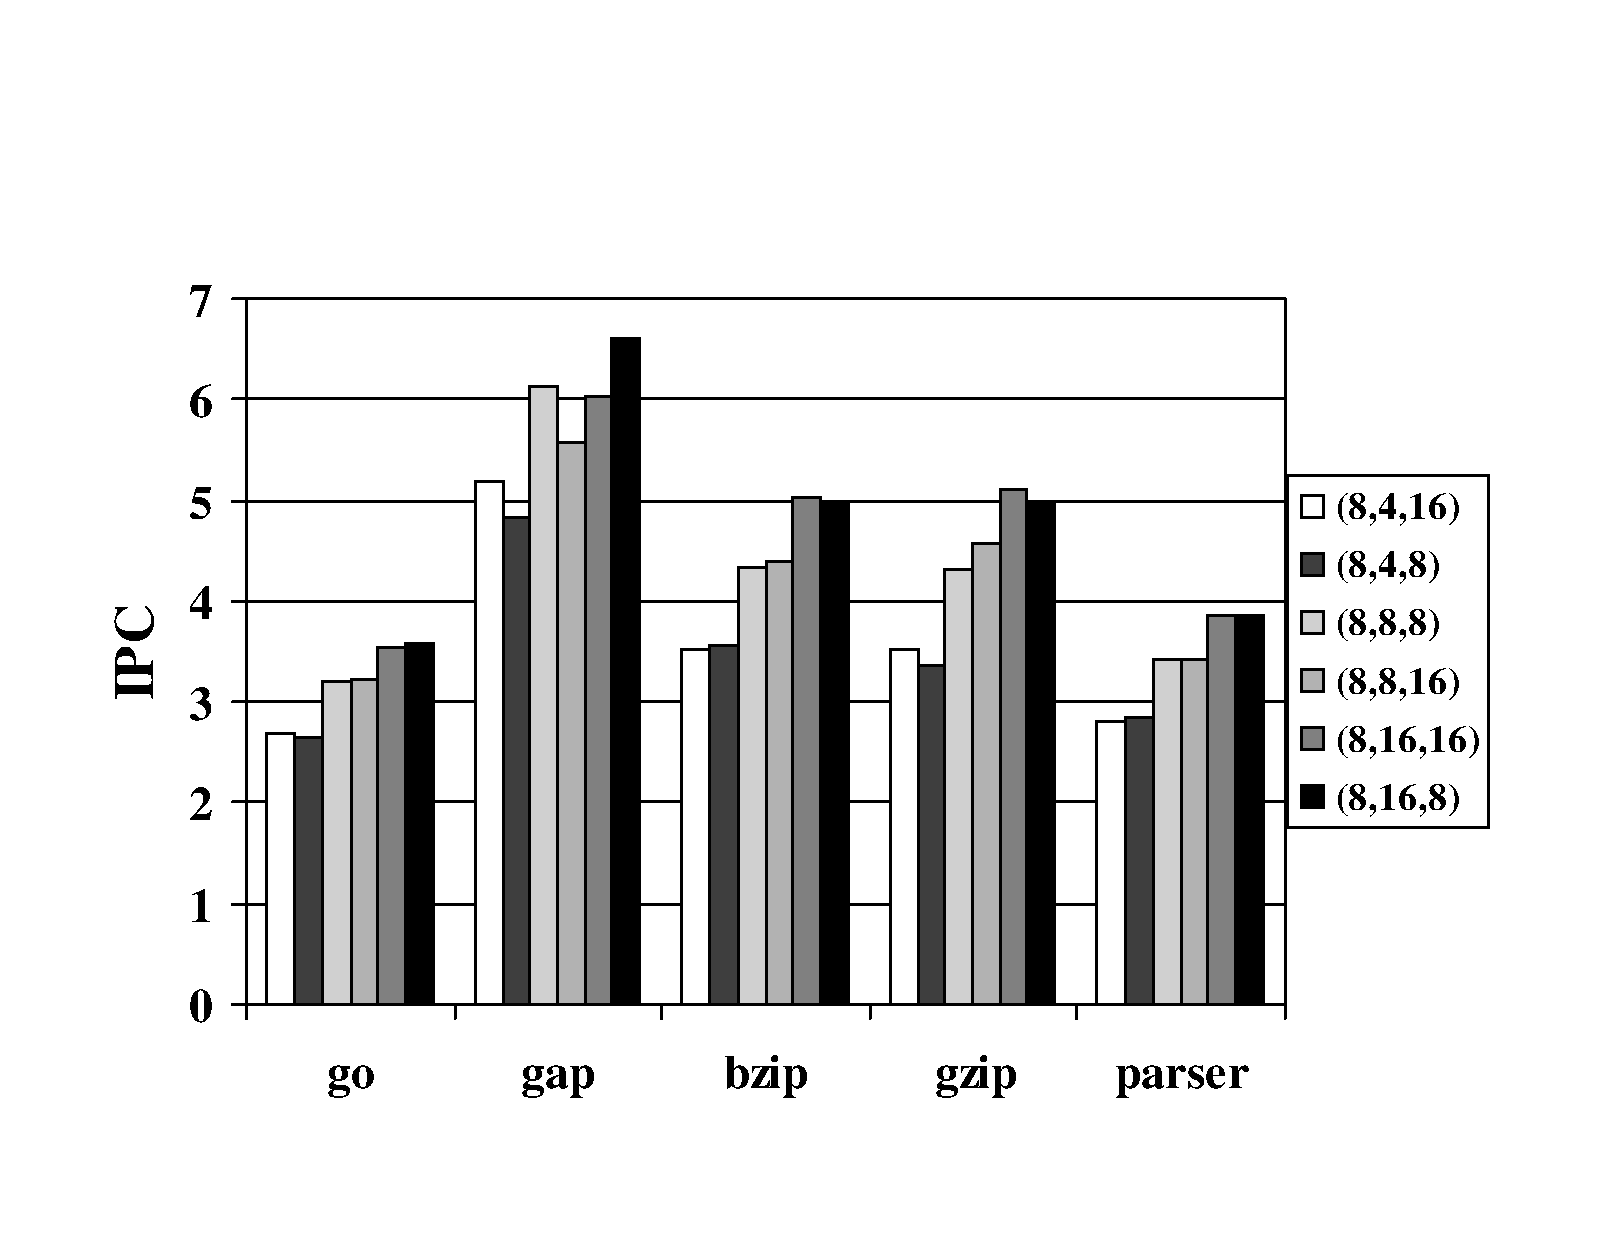
\epsfig{file=ics1.eps,width=5.8in}
\caption{{\em IPC Results for Varying Machine Configurations.} 
IPC results for several machine configurations is shown for each of
the five benchmark programs evaluated.}
\label{fig:ipc}
\end{figure}

Each of the machine configurations in Figure \ref{fig:ipc} consist of
three numbers that give: the number of sharing groups rows, the number of
active station rows per sharing group, and the number of sharing group
columns respectively.  The number of sharing group rows times the number
of active stations per sharing group is the total number of active
stations rows in a configuration.  These are all issued instructions
together in a single clock.

As can be seen from the data, the configuration of 8-16-8 provides
the best overall IPC for the configurations simulated.  This consists
of 128 active stations in each column with 16 columns.
Configuration 8-4-8 does not perform as well as 8-4-16 because it does not
have as many columns (only 8 as compared with 16 in the other configuration)
to hide the latencies of instruction execution.  Sixteen columns 
hides more instruction execution latency than Eight.  The 8-4-16
configuration performs poorly as compared with 8-8-8 because the height
of a column (the primary IPC multiplier) is only 32 and its extra
columns are not needed to hide more instruction execution latency.

Benchmark 'go' has the poorest branch prediction accuracy and that is 
the main reason for its lower IPC numbers.  
%
\subsection{Multipath Results and Discussion}
%
In this section we present data corresponding to varying the
maximum number of alternative speculative paths that are allowed.
Figure \ref{fig:figall} shows the speedup results
when multipath execution is enabled.  Results for
each benchmark program is presented.  The results for each benchmark 
consists of six groups where each group represents the results
for one of six machine configurations.

Speedups with each group of results is relative to the
single-path case with no alternative speculative paths spawned
for any conditional branches.  For each benchmark program and
for each of the six machine configurations explored, speedups
for cases with a maximum
of zero (leftmost) to seven (rightmost) additional alternative 
paths are allowed.

The most speedup is gained for 'go'.  To explain this we need to note that 
this benchmark has the lowest branch prediction rate.  Spawning disjoint 
alternative paths has the effect of reducing the branch misprediction 
penalty.

'Bzip' has the lowest speedup.  If we look at figure
\ref{fig:numbranches}  we see that branches in 'bzip' have
the highest domain size with respect to other benchmarks and
as a result there is less opportunity for spawning
disjoint paths.

We also observed a significant speedup for the 8-8-16 configuration
of 'gap'.  Our preliminary investigations suggest
that we might have captured 
a loop in our execution window that takes great speedup by elimination
the mispredictions of its branches.

\begin{figure}
\vspace{0.2 in}
\setlength{\epsfxsize}{14cm}%7
\centerline{\epsfbox{ics2.eps}}
%\centering
%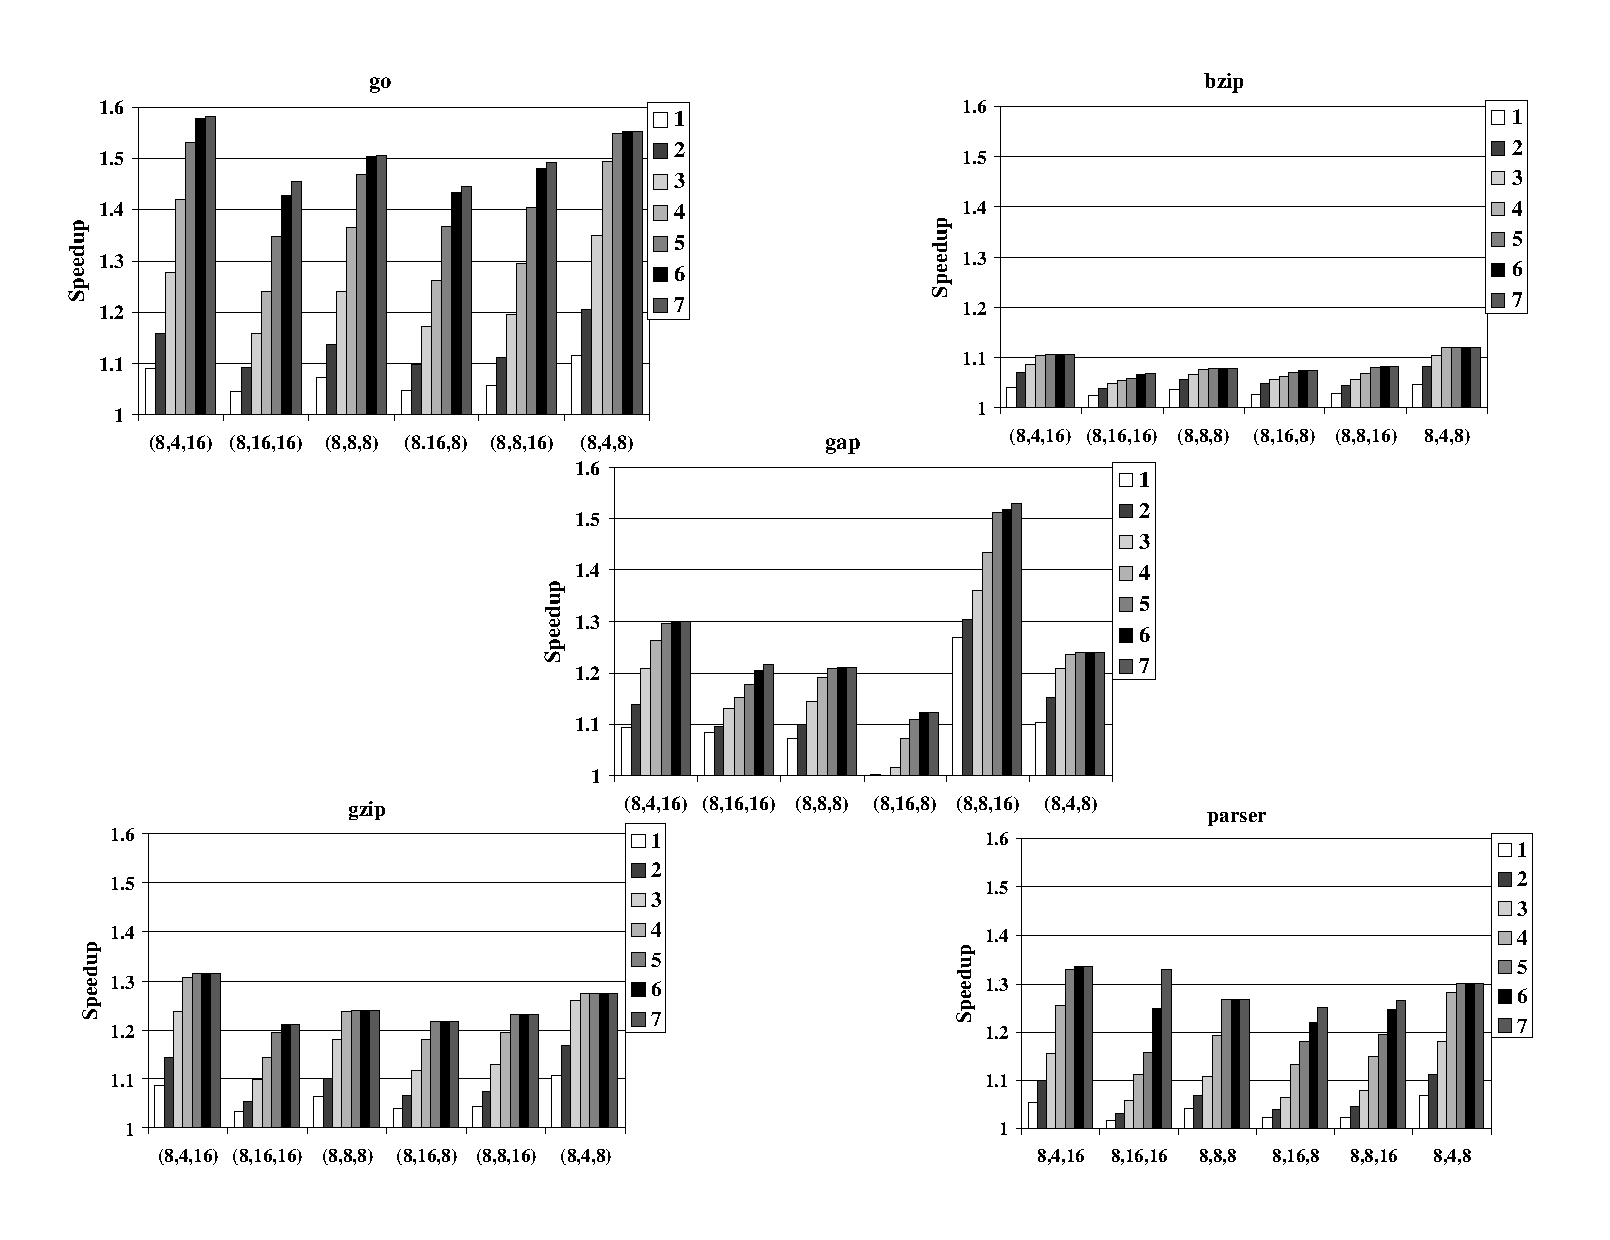
\epsfig{file=ics2.eps,width=6in}
\caption{ Multipath speedup for each benchmark.  $1-7$ denote the
spawning column. 
Speedups are relative to the Single Path execution case.}
\label{fig:figall}
\end{figure}
%
%\begin{figure}
%\centering
%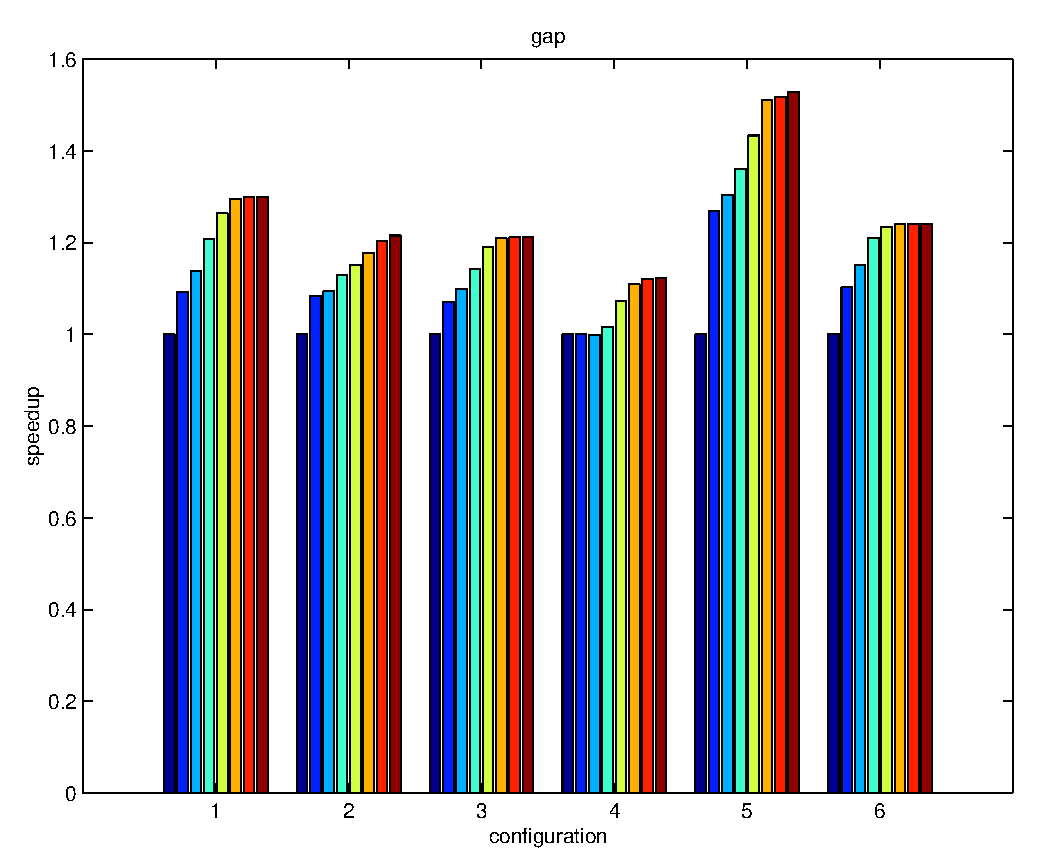
\epsfig{file=gap.eps,width=5.8in}
%\caption{{\em Multipath speedups for the BZIP2 benchmark program.} 
%IPC speedup results for several machine configurations is shown for 
%the GAP benchmark program.
%Speedups are relative to the Single Path execution case.}
%\label{fig:gap}
%\end{figure}
%
%\begin{figure}
%\centering
%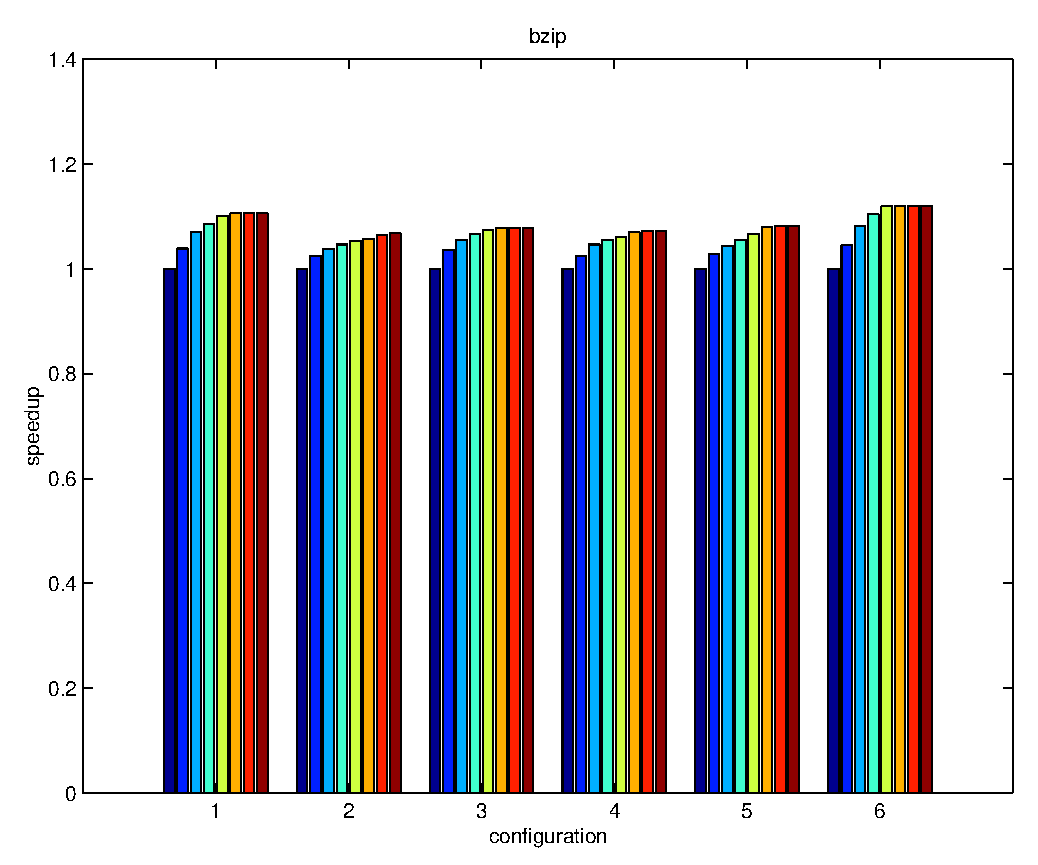
\epsfig{file=bzip2.eps,width=5.8in}
%\caption{{\em Multipath speedups for the BZIP2 benchmark program.} 
%IPC speedup results for several machine configurations is shown for 
%the BZIP2 benchmark program.
%Speedups are relative to the Single Path execution case.}
%\label{fig:bzip2}
%\end{figure}
%
%\begin{figure}
%\centering
%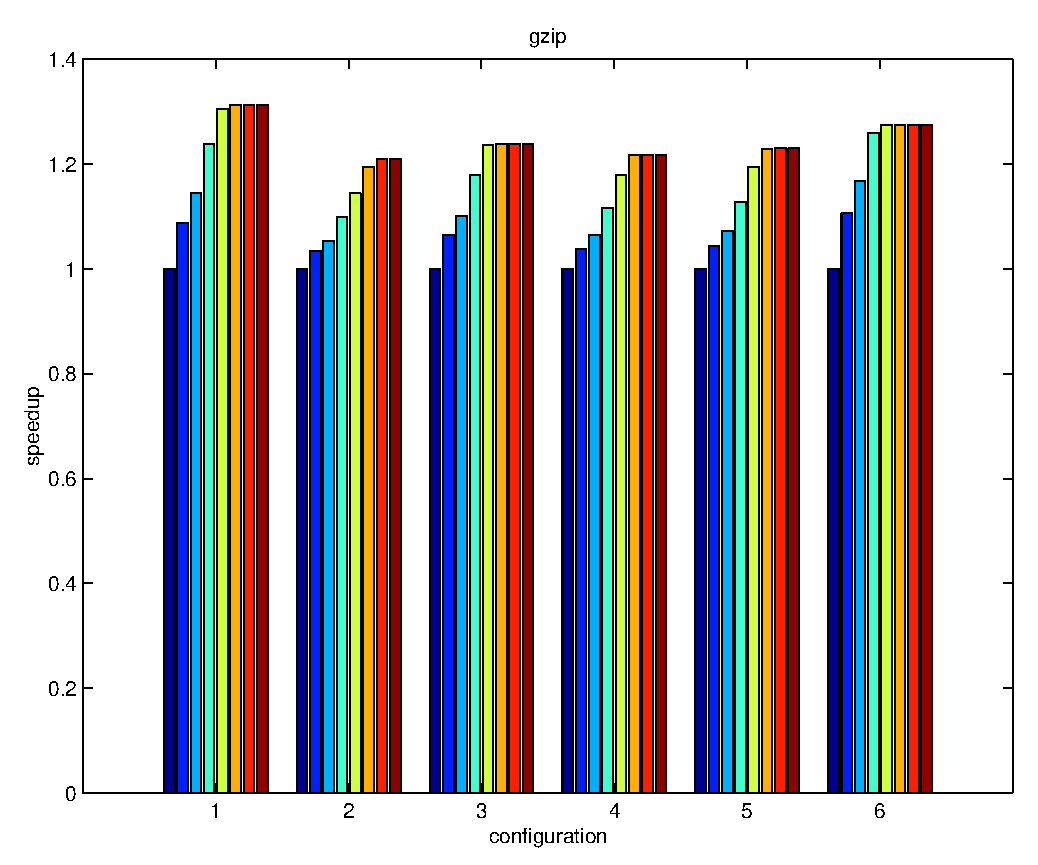
\epsfig{file=gzip.eps,width=5.8in}
%\caption{{\em Multipath speedups for the BZIP2 benchmark program.} 
%IPC speedup results for several machine configurations is shown for 
%the GZIP benchmark program.
%Speedups are relative to the Single Path execution case.}
%\label{fig:gzip}
%\end{figure}
%
%\begin{figure}
%\centering
%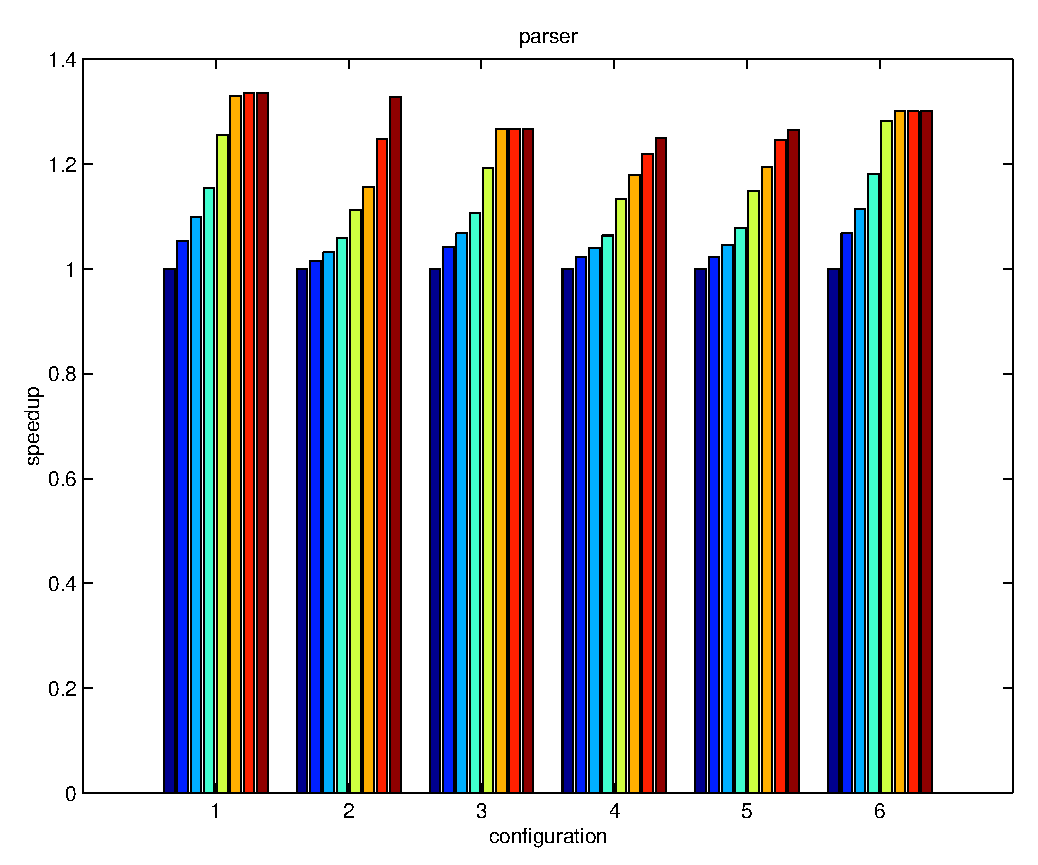
\epsfig{file=parser.eps,width=5.8in}
%\caption{{\em Multipath speedups for the BZIP2 benchmark program.} 
%IPC speedup results for several machine configurations is shown for 
%the the PARSER benchmark program.
%Speedups are relative to the Single Path execution case.}
%\label{fig:parser}
%\end{figure}
%
%
\section{Related Work}
%
Probably the most successful high-IPC machine to date is
Lipasti and Shen's Superspeculative
architecture~\cite{Lip97}, achieving an IPC of
about 7 with realistic hardware assumptions.
The Ultrascalar machine~\cite{Hen00}
achieves {\em asymptotic} scalability,
but only realizes a small amount of IPC,
due to its conservative execution model.
The Warp Engine~\cite{Cle95}
uses time tags, like Levo, for a large amount of speculation;
however their realization of time
tags is cumbersome, utilizing floating point
numbers and machine wide parameter updating.

Nagarajan et al. have proposed a {\em Grid Architecture} that
builds an array of ALUs, each with limited control, connected
by a operand network~\cite{Nag01}.  Their system achieves an IPC of 11 on
SPEC2000 and Mediabench benchmarks.  While this architecture
presents many novel ideas in attempt to reap high IPC, it
differs greatly in its interconnect strategy and register design.
They also rely on a compiler to obtain this level of IPC, whereas
the microarchitecture that we have presented does not.
%
\section{Conclusions}
%
We have presented the overview of a large-scale distributed 
microarchitecture suitable for both extracting high ILP from
sequential programs and for implementing a scheme for
multipath execution.
Our implementation of multipath execution is shown to reduce
the effects of condition branch mispredictions.
This is achieved by executing down both outcomes of those
branches that have relatively small branch domains.  These branches
would have otherwise caused largeer misprediction penalies and lower
overall execution performance in single
path only processors.

\bibliographystyle{latex8}
\bibliography{multi}

\end{document}
%
%
